%!TEX root = main.tex

\newcommand{\crosssection}{a}

\chapter{The LTE Extinction Coefficient}
\label{chapter-lte-opacity-and-emissivity}

 In this chapter, we will assume both LTE and coherent and isotropic scattering. With these assumptions, we can write the radiation transfer equation in terms of the local density, temperature, composition, and mean intensity. This is an enormous simplification. 

\newslide

In general, to solve an atmosphere, we need both the extinction coefficient $\chi$ and the source function $S_\nu$. With these, we can integrate the formal solution. 

Under the assumption of LTE, all properties of matter are properties of the local temperature, density, and composition. This includes the extinction coefficient $\chi$ and its components the absorption coefficient $\alpha$ and the scattering coefficient $\sigma$.
However, under the assumptions of both LTE and coherent and isotropic scattering, equation \ref{equation-lte-and-coherent-and-isotropic-scattering} gives
\begin{align}
S_\nu = \frac{\alpha B_\nu + \sigma J_\nu}{\alpha + \sigma}.
\end{align}
Thus, we see that the source function also depends only on the local properties of the matter, through $B_\nu(T)$, $\alpha$, and $\sigma$, and the local mean intensity $J_\nu$.

The solution for a static atmosphere in LTE and with coherent and isotropic scattering thus has two parts. The first is the determination of $\alpha$ and $\sigma$ for given properties of matter. The second is the determination of the temperature and density in a manner that satisfies the equation of transfer of radiation, thermal (often radiative) equilibrium, and mechanical (often hydrostatic) equilibrium. These two parts are coupled (since radiation determines the properties of the material and the properties of the material determine radiation), and so the solutions is typically iterative.

In this chapter, we will address the determination of $\alpha$ and $\sigma$ for a given temperature, density, and composition. We will defer solution of the global problem for a subsequent chapter.

\newslide

\section{The Extinction Coefficient in Microscopic Terms}

\begin{figure}
\begin{center}
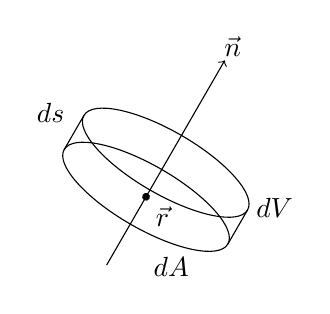
\begin{tikzpicture}
\begin{scope}[rotate=-30]
\fill[black] (0,0) circle [radius=0.05];
\draw[->] (0,-1) -- (0,2);
\draw(0,0) ellipse [x radius=1.2cm,y radius=0.4cm];
\draw(0,0.5) ellipse [x radius=1.2cm,y radius=0.4cm];
\draw(+1.2,0.5) -- (+1.2,0);
\draw(-1.2,0.5) -- (-1.2,0);
%\draw(0,3) ellipse [x radius=1.2cm,y radius=0.4cm];
%\draw(0,0) -- (-1.2,3);
%\draw(0,0) -- (+1.2,3);
\draw (0,2.2) node {$\vec n$};
\draw (0,0) node[below right] {$\vec r$};
\draw (1.3,0.3) node[above right] {$dV$};
\draw (0.6,-0.4) node[below] {$dA$};
%\draw (0.8,2) node[below right] {$d\Omega$};
\draw (-1.2,0.25) node[above left] {$ds$};
\end{scope}
\end{tikzpicture}
\end{center}
\caption{The geometry of the definition of cross-section}
\label{fig-cross-section}
\end{figure}

To proceed, we need to relate the macroscopic extinction coefficient, with its absorption and scattering components, to the microscopic properties of the material. 

Consider Figure \ref{fig-cross-section}, which shows the
volume $dV$ formed by sweeping an area $dA$ centered on
$\vec r$ thought a length $ds$ parallel to $\vec n$ which is
perpendicular to $dA$. Consider $dV$ is filled with a single type of particle with number density $n$. If these particles can interact with radiation, there is a probability that a photon that enters $dV$ in the direction $n$ will be absorbed or scattered. We define the cross-sections for absorption $\crosssection^a$ and scattering $\crosssection^s$ such that the probability of absorption or scattering of a photon is given by $n \crosssection^ads$ and $n\crosssection^sds$. (It is conventional to use $\sigma$ to denote the cross-section, but here we will use $\crosssection$ to avoid confusion with the scattering coefficient $\sigma$.)

\begin{figure}
\begin{center}
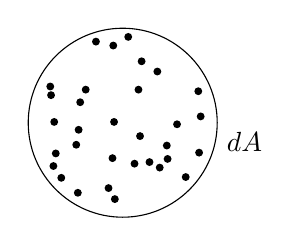
\begin{tikzpicture}
\draw(0,0) circle [radius=1.2cm];
\fill[black] (-0.11,0.01) circle [radius=0.05];
\fill[black] (0.47,-0.57) circle [radius=0.05];
\fill[black] (-0.34,1.03) circle [radius=0.05];
\fill[black] (-0.12,0.98) circle [radius=0.05];
\fill[black] (0.69,-0.02) circle [radius=0.05];
\fill[black] (0.15,-0.52) circle [radius=0.05];
\fill[black] (-0.47,0.42) circle [radius=0.05];
\fill[black] (-0.54,0.26) circle [radius=0.05];
\fill[black] (-0.91,0.35) circle [radius=0.05];
\fill[black] (-0.59,-0.28) circle [radius=0.05];
\fill[black] (0.99,0.08) circle [radius=0.05];
\fill[black] (-0.85,-0.39) circle [radius=0.05];
\fill[black] (0.44,0.65) circle [radius=0.05];
\fill[black] (0.20,0.42) circle [radius=0.05];
\fill[black] (-0.18,-0.83) circle [radius=0.05];
\fill[black] (0.34,-0.50) circle [radius=0.05];
\fill[black] (0.96,0.40) circle [radius=0.05];
\fill[black] (0.97,-0.38) circle [radius=0.05];
\fill[black] (0.07,1.09) circle [radius=0.05];
\fill[black] (0.22,-0.17) circle [radius=0.05];
\fill[black] (0.56,-0.29) circle [radius=0.05];
\fill[black] (-0.13,-0.45) circle [radius=0.05];
\fill[black] (-0.10,-0.97) circle [radius=0.05];
\fill[black] (-0.78,-0.70) circle [radius=0.05];
\fill[black] (0.57,-0.46) circle [radius=0.05];
\fill[black] (0.80,-0.69) circle [radius=0.05];
\fill[black] (-0.57,-0.89) circle [radius=0.05];
\fill[black] (-0.92,0.46) circle [radius=0.05];
\fill[black] (-0.88,-0.55) circle [radius=0.05];
\fill[black] (0.24,0.78) circle [radius=0.05];
\fill[black] (-0.56,-0.09) circle [radius=0.05];
\fill[black] (-0.87,0.01) circle [radius=0.05];
\draw (1.2,0) node[below right] {$dA$};
\end{tikzpicture}
\end{center}
\caption{The cross-section interpreted classically.}
\label{fig-classical-cross-section}
\end{figure}

\newslide

Naively, we can interpret the cross-section as the area around a particle within which the probability of interaction is 1 and outside of which the probability is 0. This is illustrated in Figure~\ref{fig-classical-cross-section}. Under this interpretation, the total area in $dV$ for interactions is the number of particles in $dV$ is the total number of particles $n dV$ multiplied by the cross-section per particle $\crosssection$. Thus, the probabilidad of an interaction is $n dV \crosssection/dA = n\crosssection ds$. This discussion helps motivate the definition of $\crosssection$, but we must remember that quantum mechanics teaches us that the interaction is probabilistic, not deterministic like this.

If we have many types of particles, the total probability of absorption or scattering is given by $(\sum_i n_i \crosssection^a_i)ds$ and $(\sum_i n_i \crosssection^s_i)ds$,  in which the index $i$ extends over all types of
particles. 

\newslide

We saw in Problem~\ref{problem-optical-depth} that the probability density function for the absorption of a photon is an exponential distribution in the optical depth $\tau$ with a mean of 1. Thus, the probability $P(<d\tau)$ that a photon is extinguished between $\tau = 0$ and $\tau = d\tau$ is
\begin{align}
P(<d\tau) &= 1 - \exp^{-d\tau}\\
&= 1 - (1 - {d\tau})\\
&= {d\tau},
\end{align}
in which we have expanded for small $d\tau$.
Now, since
\begin{align}
d\tau &= \chi ds\\
&= (\alpha + \sigma) ds,
\end{align}
by comparison to our definition of the cross-section, 
we can identify absorption and scattering coefficients as
\begin{align}
\alpha &= \sum_i n_i \crosssection^a_i(\nu)\\
\intertext{and}
\sigma &= \sum_i n_i \crosssection^s_i(\nu),
\end{align}
in which $n_i$ is the number density of particles of type $i$ and
$\crosssection^a_i(\nu)$ and $\crosssection^s_i$ are the absorption or scattering cross-section per
particle at frequency $\nu$.

Thus, we can divide the problem of determining the opacity
into two subproblems: determining the number densities $n_i$ and determining
the cross-sections $\crosssection_i$.

\newslide

\section{Distributions and Densities}

The assumption of LTE is that matter has the same state as it would in
thermodynamic equilibrium at the same density and temperature, and we can use this to determine the number densities $n_i$ of particles. 

For matter in thermodynamic equilibrium and hence also for matter in LTE,
Boltzmann's relation requires that
probability $P$ of finding a system in a given state satisfies
\begin{align}
P \propto g e^{-E/kT},
\end{align}
where $g$ is the degeneracy and $E$ is the energy of the state
\citep[pp.\ 201--203]{Reif-1965}. The constant of
proportionality can be found from the normalization condition that $\sum
P = 1$. From Boltzmann's relation and a knowledge of the degeneracies $g$
and energies $E$ of all states, we can derive the distributions of
velocities, excitation, and ionization for matter in thermal equilibrium
and, hence, in LTE.

We will typically apply the continuum approximation, that the scale of the macroscopic system is sufficiently large that the density of particles in a given state $n$ is proportional to the probability $P$ of finding the system in that state. Thus, for two states $a$ and $b$, the relative densities are given by
\begin{align}
\frac{n_a}{n_b} = \frac{P_a}{P_b}.
\end{align}

\newslide

\subsection{Velocity Distribution}

The probability $dP$ that a particle of mass $m$ has a velocity between
$v$ and $v+dv$ is given in terms of the probability distribution
function $f(v)$ by
\begin{align}
dP \equiv f(v) dv.
\end{align}
In thermodynamic equilibrium we can use the Boltzmann relation,
which gives us
\begin{align}
f(v) dv \propto g(v) dv\: e^{-E(v)/kT}.
\end{align}
If the mass of the particle is $m$, then the energy $E(v)$ is just the
kinetic energy $\frac{1}{2}mv^2$. The factor $g(v)dv$ is the number of
states between $v$ and $v+dv$. Thinking back to basic quantum mechanics,
and in particular to the the particle in a box, the density of states in
position-momentum phase space is $2/h^3$, where the 2 comes from the two
spin states of the particle (which we assume to be a spin-1/2 fermion)
and the $h^3$ from the packing of wave functions. The volume of phase
space per particle is the product of volume of position space per
particle, the inverse of the density $n$, and to the volume of momentum
space corresponding to speeds between $v$ and $v+dv$, which in turn is
proportional to $4\pi p^2 dp = 4\pi m^3v^2 dv$. So,
\begin{align}
g(v)dv = \frac{8\pi m^3 v^2}{n h^3} dv,
\end{align}
and
\begin{align}
f(v) \propto v^2 e^{-\frac{1}{2}m v^2/kT}.
\end{align}
Applying the normalization condition that $\int_0^\infty\!\!\!dv\:f(v) =
1$, we obtain the constant
of proportionality and in full we have
\begin{align}
f(v) = 4\pi\left(\frac{m}{2\pi k T}\right)^{3/2} v^2 e^{-\frac{1}{2}m v^2/kT}.
\end{align}
This is the Maxwell distribution for particle
velocities.

We can integrate the energy and the momenum flux of each particle over
the distribution to obtain the energy density $\frac{3}{2}nkT$ (assuming
ideal particles with no internal degrees of freedom) and the pressure
$nkT$. The mean kinetic energy per particle
$\frac{1}{2}m\left<v^2\right>$ is $\frac{3}{2}kT$. Thus, the RMS speed
is
\begin{align}
\left<v^2\right>^{1/2} = \left(\frac{3kT}{m}\right)^{1/2}.
\end{align}
That is, the RMS speed is proportional to the square root of the
temperature and inversely proportional to the square root of the mass.
Cooler and more massive particles have lower RMS speeds; this will be
important when we consider the Doppler broadening of lines.

\newslide

\subsection{Excitation Distribution}

In thermodynamic equilibrium, and hence in LTE, the relative probability
that an atom will be found in an excitation state $i$ is given directly
by the Boltzmann relation. By excitation state we mean an arrangement of
a fixed number of electrons forming a bound state of the atom. The
density of atoms in an given excitation state is directly proportional
to the probability that an individual atom will be found in that state.
If we denote by $n_{ijk}$ the density of atoms in excited state $i$ of
ionization state $j$ of species $k$, the population of a
state $i$ relative to the ground state is
\begin{align}
\frac{n_{ijk}}{n_{0jk}}
=
\frac{P_{ijk}}{P_{0jk}}
=
\frac{g_{ijk}}{g_{0jk}}e^{-E_{ijk}/kT},
\end{align}
where $E_{ijk}$ is the energy of the excited state above the
ground state and $g_{ijk}$ is the degeneracy of a given
state. This can obviously be extended to give the relative
populations of two excited states.

We can sum over all states to obtain the total density
$n_{jk}$ of atoms of ionization state $j$ of species $k$, obtaining
\begin{align}
n_{jk} &\equiv \sum_i n_{ijk}\\
&=n_{0jk} \sum_i \frac{n_{ijk}}{n_{0jk}}\\
&= \frac{n_{0jk}}{g_{0jk}} \sum_i g_{ijk} e^{-E_{ijk}/kT}.
\end{align}
We can write this more concisely as
\begin{align}
n_{jk} &= \frac{n_{0jk}}{g_{0jk}} U_{jk},
\end{align}
where the partition function $U_{jk}$ is defined by
\begin{align}
U_{jk} \equiv \sum_i g_{ijk} e^{-E_{ijk}/kT}
\end{align}
and the sum extends over all bound states. From this, the
population of the ground state is
\begin{align}
n_{0jk} &= \left(\frac{n_{jk}}{U_{jk}}\right) g_{0jk},\\
\intertext{and, generalizing, the population of the excitation state $i$ is}
n_{ijk} &= \left(\frac{n_{jk}}{U_{jk}}\right) g_{ijk} e^{-E_{ijk}/kT}.
\eqlabel{boltzmann-n-ijk}
\end{align}
This is a particularly useful for calculations, as it gives the
population of each state $i$ as a function of its degeneracy, the
temperature, and the density of all atoms in the ionization state.

\newslide

Disconcertingly, the partition function for an isolated atom is
divergent, as an isolated atom has an infinite number of bound states and
a upper-bound for $E_{ijk}$ is $\chi_{jk}$, the ionization potential of
ionization state $j$ of species $k$. However, in real systems this is
not a problem, since the higher bound states are increasingly spatially
extended and so at some point in a real system the interaction of the
electron with the enviroment will cause these states to cease to be
bound. For example, in an ionized gas, the presence of free electrons
causes the outermost states of an atom to be unbound. If the density of
free electrons is $n_e$, the potential of a nucleus of charge $Z$ will
be sheilded beyond the Debye length $L_\mathrm{D}$. This leads
effectively to the ionization potential being reduced by
\begin{align}
\Delta\chi &\approx \frac{Ze^2}{L_\mathrm{D}},\\
&\approx
3 \times 10^{-8}\:
Z n_e^{1/2}
T^{-1/2}~\mathrm{eV},
\end{align}
when $n_e$ and $T$ are measured in $\mathrm{cm^{-3}}$ and K. For typical
values of, say, $n_e = 10^{14}\:\mathrm{cm^{-3}}$ and $T =
10^4\:\mathrm{K}$, this lowering is only $3 \times 10^{-3}~\mathrm{eV}$,
and so it will not significantly change the ionization structure or the
position of ionization edges. However, it is enough to give only a
finite number of bound states. To see this, consider the outer wave
functions of atoms, which can be approximated by hydrogenic wave
functions with an effective nuclear charge of $Z$. In this case, the
excited state with principal quantum number $n$ lies
$13.6Z^2/n^2~\mathrm{eV}$ below the continuum. Equating this with the
energy by which the ionization potential is lowered by the free
electrons, we see that the last bound state has principal quantum number
$n_\mathrm{max}$ given by
\begin{align}
n_\mathrm{max} &\approx 2 \times 10^4\: Z^{1/2}n_e^{-1/4}T^{1/4}.\\
\intertext{At $n_e = 10^{14}\:\mathrm{cm^{-3}}$ and $T = 10^4\:\mathrm{K}$, we have}
n_\mathrm{max} &\approx 60 Z^{1/2}.
\end{align}
However, this is enough that the sum in the partition function for an
atom in a stellar atmosphere should only extend over some tens or
hundreds of states, rather than over an infinite number of states, and
the partition function should be finite. On the other hand, it is
sufficiently high that the inner wave functions, which result in
transitions at high frequencies, in the ultraviolet, optical, and
infrared, are not significantly perturbed.

Although the partition for an isolated atom is a function of temperature only,
the partition function for
an atom in an atmosphere is a function of both the temperature and the electron
density, because of the direct dependence on $T$ of the Boltzmann
factors and the indirect dependence on both $T$ and $n_e$ of the number
of bound states. However, the later dependence is weak enough that it is
usually ignored, and the number of bound states is calculated for
characteristic values of, say, $n_e = 10^{14}\:\mathrm{cm^{-3}}$ and $T
= 10^4\:\mathrm{K}$. 
The dependence of partition functions on $T$ is relatively smooth, so polynomial
approximates are more commonly used.

\newslide

\subsection{Ionization Distribution}

We can calculate the populations of different ions of the same species
in thermodynamic equilibrium, and hence LTE, by applying the Boltzmann
relation and taking into account the continuous states available to a
free electron. Consider one discrete state formed by the ground state of
a neutral atom and another state formed by the ground state of the
corresponding singly-ionized ion and an electron. The probability that
the atom is in the ground state and neutral is $P_{00k}$ and the
probability that the atom is in the ground state and ionized and the
electron has speed between $v$ and $v+dv$ is $P_{01k}f(v)dv$, where
$f(v)$ is the Maxwell distribution. The ionized atom and the electron
are independent, hence their probabilities and degeneracies are
multiplicative. Applying the Boltzmann relation we have
\begin{align}
\frac{P_{01k}f(v)dv}{P_{00k}}
=
\frac{g_{01k}g(v)dv}{g_{00k}} e^{-(\chi_{0k} + \frac{1}{2}m_e v^2)/kT}.
\end{align}
In this, $\chi_{0k}$ is the ionization potential of the ground state of
the neutral atom. 
Using the degeneracy of free electron states $g(v) =
8\pi m_e^3 v^2/n_eh^3$, obtained in our derivation of the Maxwell
distribution, and dividing by $f(v)$, we obtain
\begin{align}
\frac{n_{01k}}{n_{00k}} 
=
\frac{P_{01k}}{P_{00k}} 
=
\frac{2}{n_e}
\left(\frac{2 \pi kT m_e}{h^2}\right)^{3/2}
\frac{g_{01k}}{g_{00k}} 
e^{-\chi_{0k}/kT}.
\end{align}
We've not made any explicit reference to the lack of charge on the atom,
so we can generalize this equation to any two subsequent stages of
ionization $j$ and $j+1$, obtaining
\begin{align}
\frac{n_{0,j+1,k}}{n_{0,j,k}} 
&=
\frac{2}{n_e}
\left(\frac{2 \pi kT m_e}{h^2}\right)^{3/2}
\frac{g_{0,j+1,k}}{g_{0,j,k}} 
e^{-\chi_{jk}/kT}.
\end{align}
This gives the ionization balance between the
ground states of two subsequent ionization stages. If we use
$n_{0jk} = n_{jk} g_{0jk}/U_{jk}$, then we can write the
ionization balance between all states of two subsequent
ionization stages as
\begin{align}
\frac{n_{j+1,k}}{n_{j,k}}
&=
\frac{2}{n_e}
\left(\frac{2 \pi kT m_e}{h^2}\right)^{3/2}
\frac{U_{j+1,k}}{U_{j,k}} 
e^{-\chi_{jk}/kT}.
\eqlabel{saha-n-j}
\end{align}
This is the Saha equation. It can be applied to atoms, ion, and
electrons to give the ionization state.

We might think that we need to take into account the density of momentum states available to the the atom and ion in the same way as we take into account the density of states of the electron. However, since both have the same mass, if we include these, we discover that they cancel. 

\newslide

The Saha equation obviously states that the degree of ionization
increases with the temperature and decrease with the density of
electrons. However, we can gain a better quantitative feeling for this
by defining $n_\mathrm{S}(T) \equiv 2(2 \pi kT m_e/h^2)^{3/2}$ and writing
the Saha equation as
\begin{align}
\frac{n_{j+1,k}}{n_{j,k}} 
&=
\frac{n_\mathrm{S}}{n_e}
\frac{U_{j+1,k}}{U_{j,k}} 
e^{-\chi_{jk}/kT}.
\end{align}
The ratio of the partition function is of order unity, so we have parity
between the two ionization states when
\begin{align}
kT \approx \frac{\chi}{\ln(n_\mathrm{S}/n_e)}.
\end{align}
At $10^4\:\mathrm{K}$, $n_\mathrm{S} \approx 5 \times
10^{21}\:\mathrm{cm^{-3}}$, which is orders of magnitude
larger than the electron densities of
$10^{14}\:\mathrm{cm^{-3}}$ that are typical of stellar
atmospheres. This implies that atoms become substantially
ionized when $kT \sim \chi/20$ rather than when $kT \sim
\chi$ as might be naively expected. For 
example, hydrogen begins to be substantially ionized around $\chi/20k
\approx 8,000\:\mathrm{K}$ rather than around $\chi/k \approx
150,000\:\mathrm{K}$. Consider how different O stars would be
if their atmospheres consisted largely of neutral hydrogen!

% We can further combine this with \eqref{boltzmann-n-ijk} to determine
% $f_{ijk}$ the fraction of atoms of excited state $i$ of ionization state
% $j$ relative to all atoms of that species as
% \begin{align}
% f_{ijk}(n_e, T) &\equiv \frac{n_{ijk}}{n_k}
% = \frac{f_{jk}g_{ijk}}{U_{jk}} e^{-E_{ijk}/kT}.
% \end{align}

\newslide

\subsection{Electron Density}

In order to solve for the ionization equilibrium using the Saha
equation, we need to electron density, which is in turn
\emph{determined} by the ionization equilibrium. Once again, we have a
coupled problem.

We consider the gas as consisting of free electrons, bound electrons, and nuclei. The density of
nuclei $n_n$ is
\begin{align}
n_n = \frac{\rho}{\mu_n m_\mathrm{H}}.
\end{align}
If we define the number fraction of nuclei of type $k$ as $x_k \equiv
n_k / n_n$, the mean molecular mass per nuclei $\mu_n$ is given by
\begin{align}
\mu_n m_\mathrm{H} \equiv \sum_k x_k m_k.
\end{align}
Thus, for a given composition (set of $x_k$) and density, the density of
nuclei is known.
We can determine the free electron density from the requirement that the gas
be neutral, 
\begin{align}
n_e &= \sum_{k} \sum_{j} j n_{jk}.
\end{align}
Here we take $j= 0$ for neutral atoms, $j=1$ for singly-ionized ions,
and so on. We can define the ionization fraction of each ionization
stage $f_{jk} \equiv n_{jk} / n_k$ and write
\begin{align}
n_e
&= \sum_{k} \sum_{j} j n_k f_{jk}\\
&= n_n \sum_{k} \sum_{j} j x_k f_{jk}.
\eqlabel{neutrality}
\end{align}
We now need an expression for $f_{jk}$, and in LTE we obtain this from
the Saha equation for the ionization balance between all states of two
subsequent ionization stages,
\begin{align}
\frac{n_{j+1,k}}{n_{j,k}}
&=
\frac{n_\mathrm{S}}{n_e}
\frac{U_{j+1,k}}{U_{j,k}} 
e^{-\chi_{jk}/kT}\\
&= \frac{\tilde n_{j,k}}{n_e},
\end{align}
where $\tilde n_{j,k}(T) \equiv n_\mathrm{S}(T)
(U_{j+1,k}/U_{j,k})e^{-\chi_{jk}/kT}$. Now we can write
\begin{align}
\frac{n_{j+1,k}}{n_{0,k}}&=  \prod_{j'\le j}
\frac{n_{j'+1,k}}{n_{j',k}}
= \prod_{j'\le j} \frac{\tilde n_{j',k}}{n_e},
\eqlabel{saha-n-jk}
\end{align}
and summing over all ionization states we can obtain the total density
$n_k$ of all ions of species $k$,
\begin{align}
\frac{n_k}{n_{0k}} &\equiv \sum_{j} \frac{n_{jk}}{n_{0k}} =
\sum_{j} \prod_{ j'< j}
\frac{\tilde n_{j'k}}{n_e}.\eqlabel{saha-n-k}
\end{align}
We can combine the previous two equations
to obtain the fraction $f_{jk}$ of atoms in
ionization state $j$ relative to all atoms of that species as
\begin{align}
f_{jk} &\equiv \frac{n_{jk}}{n_k}
= \frac{\prod_{j' < j} 
\frac{\tilde n_{j'k}}{n_e}}{\sum_{j'}\prod_{j'' < j'} \frac{\tilde n_{j''
k}}{n_e}}.
\end{align}
We can now expand \eqref{neutrality} as
\begin{align}
n_e &= n_n \sum_{k} \sum_{j} j x_k f_{jk}\\
&= n_n \sum_{k} \sum_{j}
\left(
j x_k 
\frac{\prod_{j' < j} 
\frac{\tilde n_{j'k}}{n_e}}{\sum_{j'}\prod_{j'' < j'} \frac{\tilde n_{j''
k}}{n_e}}
\right).
\label{equation-ne}
\end{align}
Since $n_n$ and $T$ are known, this is an implicit equation for $n_e$.
It can be rearranged as a polynomial in $n_e$, whose order is the number of stages of ionization present (i.e., quadratic for neutral and single-ionized species, cubic for neutral, singly-ionized, and doubly-ionized species, and so on).
Except in special cases, the order will be sufficiently high that cannot solve for $n_e$ directly but
instead we must solve for $n_e$ iteratively, using standard algorithms
such the Newton-Raphson method \cite[chapter 10]{Press-1992}.

\newslide

\subsection{Application to Hydrogen}

The electron density in a pure hydrogen gas can be solved analytically
if we consider only neutral and singly-ionized hydrogen and ignore
$\mathrm{H}^-$ and all molecules. In this case, $x_1 = 1$, $n_n = n_{01}
+ n_{11} = n_1$, so Equation (\ref{equation-ne}) becomes 
\begin{align}
n_e = n_1 \frac{\frac{\tilde n_{01}}{n_e}}{1 + \frac{\tilde
n_{01}}{n_e}},
\end{align}
which can be rearranged to give the quadratic equation
\begin{align}
n_e^2 + \tilde n_{01} n_e - \tilde n_{01} n_1 = 0.
\end{align}
We anticipated a quadratic equation, because we have two stages of ionization present. 

This equation can also be obtained by considering conservation of nuclei,
\begin{align}
n_{01} + n_{11} = n_1,
\end{align}
the requirement that the gas be electrically neutral,
\begin{align}
n_e = n_{11},
\end{align}
and the Saha equation for the ionization of neutral hydrogen,
\begin{align}
\frac{n_{11}}{n_{01}} = \frac{\tilde n_{01}}{n_e}.
\end{align}
If these three equations are solved simultaneously for $n_e$ in terms of $n_1$ and $\tilde n_{01}$, one obtains the same quadratic equation.

The quadratic equation can be solved exactly to give
\begin{align}
n_e = \frac{\tilde n_{01}}{2}
\left[\left(1 + \frac{4 n_1}{\tilde n_{01}}\right)^{1/2} - 1\right].
\end{align}

To understand the behavior of the gas, we will consider the fraction of ionization $f_{11} = n_{11} / n_1$. This is the fraction of the hydrogen atoms that are ionized to $\mathrm{H}^+$. Since here we have $n_{11} = n_e$, $f_{11}$ is given by
\begin{align}
f_{11} = \frac{\tilde n_{01}}{2n_1}
\left[\left(1 + \frac{4 n_1}{\tilde n_{01}}\right)^{1/2} - 1\right].
\end{align}
In the limits of high density and low temperature (i.e., $n_1 \gg \tilde n_{01}$) and low density or high temperature (i.e., $n_1 \ll \tilde n_{01}$), we have 
\begin{align}
f_{11} \approx
\left\{
\begin{array}{ll}
\left(\frac{\tilde n_{01}}{n_1}\right)^{1/2}&\mbox{for $n_1 \gg \tilde n_{01}$, and}\\
1 - \frac{n_1}{\tilde n_{01}}&\mbox{for $n_1 \ll \tilde n_{01}$.}\\
\end{array}
\right.
\end{align}
We see that in the limit of high density and low temperature, $f_{11} \approx (\tilde n_{01}/n_1)^{1/2} \ll 1$ and the gas is almost completely neutral, whereas in the limit of low density and high temperature $f_{11} \approx 1$ and the gas is almost completely ionized. These limits correspond to our expectations based on the behavior of the Saha equation with temperature and density.

% Note that the expression for $f_{jk}$ is non-linear in the electron
% density $n_e$. For example, the fractions of helium in the neutral,
% single-ionized, and double-ionized states are
% \begin{align}
% f_{02} &= \frac{1}{1 + \frac{\tilde n_{02}}{n_e} + \frac{\tilde n_{02}
% \tilde n_{12}}{n_e^2}}
% = \frac{n_e^2}{n_e^2 + \tilde n_{02}n_e + \tilde n_{02} \tilde n_{12}}\\
% f_{12} &= \frac{\frac{\tilde n_{02}}{n_e}}{1 + \frac{\tilde n_{02}}{n_e} + \frac{\tilde n_{02}
% \tilde n_{12}}{n_e^2}}
% = \frac{\tilde n_{02}n_e}{n_e^2 + \tilde n_{02}n_e + \tilde n_{02} \tilde n_{12}}\\
% f_{22} &= \frac{\frac{\tilde n_{02}
% \tilde n_{12}}{n_e^2}}{1 + \frac{\tilde n_{02}}{n_e} + \frac{\tilde n_{02}
% \tilde n_{12}}{n_e^2}}
% = \frac{\tilde n_{02} \tilde n_{12}}{n_e^2 + \tilde n_{02}n_e + \tilde
% n_{02} \tilde n_{12}}
% \end{align}

% The condition of hydrostatic equilibrium (or, more generally, the
% dynamics of the atmosphere) will normally lead to a constraint on the
% gas pressure at each point in the atmosphere. The gas pressure $P_g$ is
% related to the density $\rho$ and the temperature $T$ through the
% equation of state. At the densities and temperatures encountered in
% stellar atmospheres, an ideal gas is a good approximation, and we have
% \begin{align}
% P_g = nkT,
% \end{align}
% where $n$ is the total particle density, or
% \begin{align}
% P_g = \frac{\rho kT}{\mu m_H}
% \end{align}
% where $\rho$ the mass density and $\mu$ the mean molecular mass.
% However, in a stellar atmosphere there is one significant complication:
% the mean molecular mass $\mu$ depends on the temperature. This is
% because because the gas can change its ionization state as the
% temperature or density changes, and when an atom is ionized one particle
% becomes two particles, which reduces the mean molecular weight. The
% contribution to the pressure doubles, while the contribution to the mass
% remains constant.

% We deal with this complication by using the temperature $T$ to convert
% the constraint on the pressure into a constraint on the total number
% density of particles $n$. We then write this as the sum of the density
% of free electrons $n_e$ and the density of nuclei $n_n$, where this
% covers all atoms and ions of all species.\comment{We can look at this as
% having a system of equations for the $n_{jk}$ and $n_e$ and eliminating
% the former to obtain the latter.} We now have
% \begin{align}
% n 
% &= n_e + n_n.
% \end{align}
% From the requirement that the gas be neutral, the electron
% density can be written as
% \begin{align}
% n_e &= \sum_{k} \sum_{j} j n_{jk},
% \end{align}
% where $n_{jk}$ is the density of ions in ionization stage $j$ of species
% $k$. We can define the number fraction of each species $x_k = n_k / n_n$
% and the ionization fraction of each ionization stage $f_{jk} = n_{jk} /
% n_k$. After this, we can write
% \begin{align}
% n_e
% &= \sum_{k} \sum_{j} j n_k f_{jk}\\
% &= \sum_{k} \sum_{j} j n_n x_k f_{jk}
% \end{align}
% and if we factor out $n_n = n - n_e$ we obtain
% \begin{align}
% n_e = (n - n_e) \sum_{k} \sum_{j} j x_k f_{jk}.
% \eqlabel{neutrality}
% \end{align}

\newslide

\section{Radiative Processes}

\subsection{Bound-Bound Transitions}

Bound-bound transitions arise between two bound states, each
of which has a more-or-less well-defined energy and as such
give rise to lines. Bound-bound transitions occur as
spontaneous emissions from an upper state to a lower state,
absorptions from a lower state to an upper state, and
stimulated emissions from an upper state to a lower state.

\subsubsection{Einstein Coefficients}

At the atomic level we have spontaneous emission, stimulated
emission, and absorption. The processes of spontaneous
emission and absorption are straightforward and can be
represented by
\begin{align}
\reversiblereaction{X_u}{X_l + \gamma},
\end{align}
with $X_u$ representing the upper level and $X_l$ the lower
level. Stimulated emission is not so obvious. It occurs when
a photon ``stimulates'' a particle in the upper state to
decay to the lower state and emit a photon. It can be
represented by
\begin{align}
\reaction{X_u + \gamma}{X_l + 2\gamma}.
\end{align}
In his work on black body radiation, Einstein was forced to
postulate stimulated emission to give the correct form of
the Planck function. Later it was shown to arise naturally
from the statistics of massless bosones particles like the
photon, as the probablity of emission into a state is
proportional to 1 plus the number of bosons in that state
\cite[sections 61 and 62]{Dirac-1958}. The part proportional to
1 corresponds to spontaneous emission and part proportional
to the number of bosons corresponds to stimulated emission.
The photon created by stimulated emission has the same
direction, frequency, and polarization as the stimulating
photon.

The Einstein coefficients $A_{ul}$, $B_{ul}$, and $B_{lu}$
quantify the strength of a line in terms of spontaneous
emission, stimulated emission, and absorption. The
coefficients are defined in terms of the probability per
unit time of a transition:
\begin{enumerate}
\item
The probability of a spontaneous emission per unit time per
unit solid angle per unit frequency for an atom in the upper
state is
\begin{align}
\frac{1}{4\pi}A_{ul}\psi.
\end{align}
The function $\psi(\nu)$ is the emission profile
and is normalized by
\begin{align}
\int_0^\infty\!\!\!d\nu\:\psi &\equiv 1.
\end{align}
\item
The probability of a stimulated emission per unit time per
unit solid angle per unit frequency  for
an atom in the upper state is 
\begin{align}
\frac{1}{4\pi}B_{ul}\psi I_\nu.
\end{align}
\item
The probability of an absorption per unit time per
unit solid angle per unit frequency  for an atom
in the lower state is \begin{align}
\frac{1}{4\pi}B_{lu}\phi I_\nu.
\end{align}
The function $\phi(\nu)$ is the absorption profile
and is normalized by
\begin{align}
\int_0^\infty\!\!\!d\nu\:\phi &\equiv 1.
\end{align}
\end{enumerate}
Other definitions of the Einstein coefficients have the
probabilities being the product of the coefficients and the
energy density $u_\nu$, which leads to $B_{ul}$ and $B_{lu}$
differing by a factor of $c/4\pi$ from those defined here.

In the definition of the Einstein coefficients, we have
carefully distinguished between the emission profile
$\psi$ and the absorption profile $\phi$. In
thermodynamic equilibrium, the principal of detailed balance
requires that emissions and absorptions at each frequency
exactly balance, and so the emission profile $\psi$ and
absorption profile $\phi$ must be equal. More generally,
when we have complete redistribution (that is, no
correlation between the frequencies of the absorbed or
emitted photons) or when the specific intensity is constant
over the line, the absorption and emission profiles will be
equal. Complete redistribuition is a good approximation for
lines in which the Doppler core dominates, and in these
cases we can assume that the profiles are identical.

However, when we have partial redistribution (that is,
correlations between the frequencies of the absorbed and
emitted photons) coupled with changes of the specific
intensity over the line, the absorption and emission
profiles can be different. By their very nature, lines are
places where the specific intensity can vary dramatically,
so we need to be wary of partial redistribution. It can
occur in strong lines that are dominated by their wings. In
a strong line, a photon is absorbed and then rapidly
re-emited; in the wing of the line, the frequency of the
emitted photon is strongly correlated with the frequency of
the absorbed photon. Roughly, then, the emission profile
will be the product of the absorption profile and the mean
intensity. If the mean intensity varies significantly over
the line, for example, being small in the core and large in
the wings, the emission profile can be very different from
the absorption profile. Nevertheless, dealing with the
difference between the absorption and emission profiles
creates significant additional complexity, and for this
reason we'll often assume that the two are equal even when
this is cannot be justified on physical grounds.

The Einstein coefficients are related by the Einstein
Relations, which we can derive by considering the behaviour
of a population of atoms in thermodynamic equilibrium. In
thermodynamic equilibrium we have detailed balance, and so
the rate of upward radiative transitions at a given
frequency and in a given direction must be exactly balanced
by the rate of downward transitions at the same frequency
and in the same direction. The rate of a transition from one
state to a second is simply the number of atoms in the first
state multipled by the probability per unit time of a
transition to the second state. Thus, if the density of
atoms in the upper  states is $n_u$ and the density of
atoms in the lower state is $n_u$, then we must have
\begin{align}
n_u(A_{ul} + B_{ul}I_\nu)\psi 
=
n_l B_{lu}\phi I_\nu.
\end{align}
Furthermore, detailed balance requires that the emission and
absorption profiles be equal and we also have $I_\nu =
B_\nu$, and so
\begin{align}
n_u(A_{ul} + B_{ul} B_\nu)
=
n_l B_{lu}B_\nu.
\end{align}
We can rearrange this to obtain 
\begin{align}
B_\nu = \frac{A_{ul}/B_{ul}}{(n_l/n_u)(B_{lu}/B_{ul}) - 1}.
\end{align}
Since in thermodynamic equlibrium the level populations are
given by a Boltzman distribution, $n_l/n_u = (g_l/g_u)
e^{E/kT}$, where $E = h\nu$ is the energy difference between
the levels, we have
\begin{align}
B_\nu = \frac{A_{ul}/B_{ul}}{(g_l/g_u)
(B_{lu}/B_{ul})e^{h\nu/kT} - 1}.
\end{align}
On the righthand side, the only variables are $\nu$ and $T$;
all other quantities are constants or properties of the atom
that are independent of temperature or frequency. Thus, in
order for this equation to hold at all temperatures, we must
have
\begin{align}
g_u B_{ul} = g_l B_{lu}
\end{align} 
and 
\begin{align}
A_{ul} = \frac{2h\nu^3}{c^2} B_{ul}.
\end{align}
These equations are known as the Einstein relations. They
show that a line has a unique intrinsic strength -- which we
can choose to measure by any one of the three Einstein
coefficients. The intrinsic strength of a line is ultimately
derived from the dipole matrix element between the two
states.

\subsubsection{The Line Emission and Absorption Coefficients}

We can define the contribution of a single line to the
emission coefficient $j_\nu(\nu)$ to be
$j_\nu^\mathrm{L}(\nu)$ and the contribution of a single
line to the absorption coefficient $\alpha(\nu)$ to be
$\alpha^\mathrm{L}$.

The Einstein coefficients give the probability of a transition per unit
time per atom. If we multiply them by the density of atoms in the
initial state, $n_u$ or $n_l$, and by the energy of the transition,
$h\nu$, we obtain the rate of exchange of energy between the radiation
field and matter per unit volume per unit solid angle per unit
frequency. Depending on the direction of the exchange, these are just
the absorption and emission coefficients. Thus, we have
\begin{align}
j_\nu^\mathrm{L} = \frac{h\nu}{4\pi} A_{ul} n_u \psi
\end{align}
and
\begin{align}
\alpha^\mathrm{L} = \frac{h\nu}{4\pi} (B_{lu} n_l
\phi - B_{ul} n_u\psi).
\end{align}
Note that we consider stimulated emission to be a negative
absorption. This is mathematically convenient, as it ensures
that the emission remains independent of direct dependence
on the specific intensity and the processes that depend
directly on the specific intensity are gathered in the
absorption coefficient. Physically, the photon created by
stimulated emission has the same direction, frequency, and
polarization as the stimulating photon and so stimulated
emission can be thought of a photon passing an atom and the
result being two photons rather than none, the result for
absorption.

There is one difference, however, betweeen absorption and
stimulated emission. The probability for stimulated emission
is proportional to the emission profile $\psi$ whereas
probability of absorption is proportional to the absorption
profile $\phi$. In general, these need not be equal --
for example, the absorbing and emitting atoms might have
different velocity distributions -- and so in general
stimulated emission does not correspond exactly to negative
absorption. Nevertheless, we commonly assume that the
difference between the profiles is not important. In this
case, stimulated emission can be treated exactly as a
negative absorption.

We can write the contribution of a single line to the
emission coefficient $j_\nu(\nu)$ and the absorption
coefficient $\alpha$ as
\begin{align}
j_\nu^\mathrm{L}(\nu) &\equiv j^\mathrm{L} \psi(\nu)\\
\intertext{and}
\alpha^\mathrm{L}(\nu) &\equiv \alpha^\mathrm{L} \phi(\nu).
\end{align}
Here we have ignored the difference between the profiles for
absorption and stimulated emission. Because of the
normalization of $\psi$ and $\phi$, we have
\begin{align}
j^\mathrm{L} &= \int_0^\infty\!\!\!d\nu\:j_\nu^\mathrm{L}(\nu)\\
\intertext{and}
\alpha^\mathrm{L} &= \int_0^\infty\!\!\!d\nu\:\alpha^\mathrm{L}(\nu),
\end{align}
and so $j^\mathrm{L}$ and $\alpha$ are known as the
integrated line emission and aborption coefficients. We can
now see that $j^\mathrm{L}$ and $\alpha$ characterize
the strength of a line, whereas $\psi$ and $\phi$
characterize its shape. In terms of the Einstein
coefficients, the intergrated coefficients are given by
\begin{align}
j^\mathrm{L} &= \frac{h\nu}{4\pi} A_{ul} n_u\\
\intertext{and}
\alpha^\mathrm{L} &= \frac{h\nu}{4\pi} (B_{lu} n_l - B_{ul}
n_u).
\end{align}

We can use the Einstein relation that $g_l B_{lu} = g_u
B_{ul}$ to write the integrated emission coefficient as
\begin{align}
\alpha^\mathrm{L} &= \frac{h\nu}{4\pi} B_{lu} n_l \left(1 - 
\frac{g_l n_u}{g_u n_l}\right).
\end{align}
This has the form of the coefficient for true absorption
multiplied by a correction factor that accounts for
stimulated emission. If $n_u/n_l > g_u/g_l$ we have a
\emph{population inversion} and the absorption coefficient
becomes negative. In this case, stimulated emission more
than compensates for absorption, and as light passes through
the medium it will be amplified by stimulated emission,
producing a laser or maser (Light or Microwaves Amplified by
the Stimulated Emission of Radiation). This can be seen from
the solution to the equation of radiative transfer: when the
extinction coefficient is positive, the optical depth also
is positive, the $e^{-\tau}$ factor is less than 1 and
diminishes incoming light; when the extinction coefficient
is negative, when the optical depth is also negative, the
$e^{-\tau}$ factor is greater than 1 and amplifies incoming
light. Masers are often seen in the dense circumstellar
environments of young and old stars.

\begin{figure}
\centering
\input figures/stimulated-emission.tex
\caption{The LTE correction factor for stimulated emission $1 -
e^{-h\nu/kT}$ at $10^4$ K (solid line) compared to a scaled
version of the Planck function (dotted line). Also shown (dashed, right to left) are
the frequencies of Ly$\alpha$, H$\alpha$, Pa$\alpha$,
Br$\alpha$, and Pf$\alpha$.}
\label{figure-stimulated-emssion}
\end{figure}

In LTE the populations of the upper and lower states have a
Boltzmann distribution, then $n_u / n_l = g_u/g_l
e^{-h\nu/kT}$, and we have
\begin{align}
\alpha^\mathrm{L} &= \frac{h\nu}{4\pi} B_{lu} n_l 
(1 - e^{-h\nu/kT}).
\end{align}
The correction factor is thus always positive; we cannot
have a maser when the populations are given by a Boltzmann
distribution. To create a maser, we need non-LTE conditions.
Figure \ref{figure-stimulated-emssion} compares the LTE
correction factor for stimulated emission $1 - e^{-h\nu/kT}$
at $10^4$ K against the Planck function. It also shows the
positions of Ly$\alpha$ ($n = 2\rightarrow1$, 1216 {\Angstrom}),
H$\alpha$ ($n=3\rightarrow2$, 6563 {\Angstrom}), Pa$\alpha$
($n=4\rightarrow3$, 1.875 {\micron}), Br$\alpha$ ($n=5\rightarrow4$, 4.051
{\micron}), and Pf$\alpha$ ($n=6\rightarrow5$, 7.458 {\micron}). It
shows that the correction for stimulated emission is
negligible in the Wien tail (e.g., for Ly$\alpha$), small
but nonetheless not negligible close the peak of the Planck
function (e.g., for H$\alpha$), and large in the
Rayleigh-Jeans tail (e.g., for Pa$\alpha$, Br$\alpha$, and
Pf$\alpha$).

In the Rayleigh-Jeans tail we have $1 - e^{-h\nu/kT} \approx
h\nu/kT$, which is small; stimulated emission almost exactly
balances absorption. The increasing importance of stimulated
emission means that only a small
over population of the upper level relative to its LTE value
is sufficient to cause the line to mase. For example, in
\ion{H}{II} regions the levels of hydrogen have non-LTE
populations and recombination lines such as H72$\alpha$
($n=73\rightarrow72$), which has a correction factor of only $8.2\times10^{-5}$ at $10^4$ K, are
observed to mase because even a slight departure of LTE is
enough to cause a population inversion.

\subsubsection{Permitted and Forbidden Transitions}

In astrophysics we distinguish between permitted and
forbidden transitions. The lines observed in stellar
atmospheres are almost exclusively permitted lines.
Permitted transitions arise from electric dipole transitions
and have a high probability, with $A_{ul}$ typically being of order unity, whereas forbidden transitions arise from electric
quadrupole or magnetic dipole transitions and have lower
probabilities, with $A_{ul}$ typically being $10^{-3}$ or less. 
The rules on the changes in quantum
number that produce permitted rather than forbidden
transitions are known as selection rules.

Forbidden lines are rarely seen in absorption because they are so weak;
recall that $\alpha^\mathrm{L}$ is directly proportional to $B_{lu}$,
which in turn is directly proportional to $A_{ul}$. Thus, forbidden
absorption lines will be many orders of magnitude weaker than permitted
absorption lines, and are only detectable in spectral with excellent signal-to-noise
ratios.

Stellar emission lines most often arise in the chromosphere
and winds.  Permitted lines
are again typically the strongest. The probability of a forbidden transition is
relatively low, so an atom has to spend a relatively long
time (typically $A_{lu}^{-1}$ or longer than 1000~s) in an excited state
before it can emit by a forbidden transition. In this time,
at the relatively high densities in the photosphere,
chromosphere, and even the wind, the atom is likely to
undergo a collision, which can de-excite it without emitting
a photon. We say that at these high densities the lines are
\emph{collisionally quenched}.

\subsubsection{Oscillator Strengths}

Absorption lines can be modelled classically as the
interaction of photons with oscillating electrons. The
result is adequate in some aspects, but its major failing of
the model is that it predicts that all lines have the same
strength. This is because it attributes only one characteristic -- energy
difference -- to a transition. However, quantum mechanics shows us that an equally important characteristic is the dipole element.

An ad hoc solution to this problem is to attribute an
\emph{oscillator strength} to each line, and to arbitrarily
modify the model line strengths by multiplying them by this
factor. The oscillator strengths are determined by requiring
that the modified model line strengths match the the true
line strengths, determined from quantum mechanical
calculation, laboratory experiment, or astrophysical
observation. The classical absorption oscillator strength
$f_{lu}$ is defined in terms of Einstein coefficient
$B_{lu}$ by
\begin{align}
B_{lu} = \frac{4\pi^2 e^2}{h\nu m_e c} f_{lu}.
\end{align}
An equivalent emission oscillator strength $f_{ul}$ can be
defined in terms of $B_{ul}$. Oscilator strengths are always
given in the combination $gf$, the degeneracy of the
originating state multiplied by the oscilator strength for
the transition, as the Einstein relation that $g_u B_{ul} =
g_l B_{lu}$ implies that $g_u f_{ul} = g_l f_{lu}$. The
oscilator strength has no direct physical meaning beyond
quantifying the relative strengths of lines; it is simply
the empirical correction factor we have to apply to an
incorrect theory in order to obtain the correct result.
Nonetheless, for reasons of precedent, line strengths are
still often given in terms of the oscillator strengths.

From the definition of the oscilator strength, we can see
that the integrated absorption coefficient is given by
\begin{align}
\alpha^\mathrm{L} =  n_l f_{lu}\left(\frac{\pi e^2}{m_e c}\right)\left(1 - \frac{g_l n_u}{g_u n_l}\right),
\end{align}
in which the last factor is the correction for stimulated
emission, and the integrated emission coefficient is given
by
\begin{align}
j^\mathrm{L} = \left(\frac{2h\nu^3}{c^2}\right)n_u
f_{ul}\left(\frac{\pi e^2}{m_e c}\right).
\end{align}

\subsubsection{Determination of Oscillator Strengths}

\comment{Quantum mechanical calculations. Exact for H and
H-F for others. R-L p.\~276 say why we need good wave functions. Coulomb
approximation? Laboratory measurements. Observations. Sum rules. Give
table of oscillator strengths for some common lines.}

\subsection{Bound-Free and Free-Bound Transitions}

\comment{The stuff in Osterbrock on heavy-element ionization
and dielectronic recombination is good.}

Bound-free radiative transitions correspond to
photoionizations and free-bound radiative transitions to
recombinations. They can be represented by
\begin{align}
\reversiblereaction{X^+ + e^-}{X + \gamma}.
\end{align}
As with bound-bound transitions, there is a stimulated
recombination process which can be represented by
\begin{align}
\reaction{X^+ + e^- + \gamma}{X + 2\gamma}.
\end{align}

Rate of photoionizations per unit volume per unit frequency per unit
solid angle is
\begin{align}
\frac{1}{h\nu} \crosssection_{bf} (1 - e^{-h\nu/kT}) I_\nu n_n
\end{align}

\comment{The second part is stimulated recombination. I'm not sure why
it has exactly this form.}

Rate of radiative recombinations per unit volume per unit velocity is
\begin{align}
n_i n_e \crosssection_{fb}(v) f(v) v
\end{align}

\subsubsection{Milne Relations}

In TE and using detailed balance, we have
\begin{align}
\frac{\crosssection_{bf}}{\crosssection_{fb}}
&= 
\frac{n_i n_e}{n_n}
\frac{h\nu f(v) v}{4\pi (1-e^{-h\nu/kT}) B_\nu}
\frac{dv}{d\nu}\\
&=
\frac{n_i n_e}{n_n}
e^{h\nu/kT}
\frac{f(v) vc^2}{8\pi \nu^2}
\frac{dv}{d\nu}\\
\intertext{and $h\nu = mv^2/2 + \chi$, so $hd\nu = m v dv$, so}
\frac{\crosssection_{bf}}{\crosssection_{fb}}
&=
\frac{n_i n_e}{n_n}
e^{h\nu/kT}
\frac{f(v) h c^2}{8\pi m_e \nu^2}.
\end{align}
But Maxwell says
\begin{align}
f(v) = 4\pi \left(\frac{m_e}{2\pi k T}\right)^{3/2} v^2 e^{-mv^2/2kT}
\end{align}
and Saha says
\begin{align}
\frac{n_i n_e}{n_n}
=
2
\left(\frac{2\pi m_e k T}{h^2}\right)^{3/2}
\frac{g_i}{g_n} 
e^{-\chi/kT}
\end{align}
Thus,
\begin{align}
\frac{\crosssection_{bf}}{\crosssection_{fb}}
&= 
\frac{m_e^2c^2v^2}{\nu^2 h^2}
\frac{g_i}{g_n}
e^{(h\nu -mv^2/2 - \chi)/kT}
\intertext{and since $h\nu = mv^2/2 - \chi$,}
\frac{\crosssection_{bf}}{\crosssection_{fb}}
&= 
\frac{g_i}{g_n}
\frac{m_e^2c^2v^2}{\nu^2 h^2}.
\end{align}

\subsection{Emission and Absorption Coefficients}

As above, 
\begin{align}
\alpha^{bf} = n_n \crosssection_{bf}(1 - e^{-h\nu/kT})
\end{align}
and
\begin{align}
j_\nu^{bf} &= \frac{h\nu}{4\pi} n_i n_e \crosssection_{fb}(v) f(v)
         v dv/d\nu
\end{align}

\subsubsection{Determination}

Determination again proceeds mainly from QM using similar
methods to those for BB transitions. Having obtained
$\crosssection_{bf}$, we can use the Milne relation to obtain
$\crosssection_{bf}$.

For hydrogen-like transition, ionization from a state with a
given $n$ has
\begin{align}
\crosssection_{bf} = \left(\frac{64\pi n}{3\sqrt{3} Z^2}\right)
\alpha a_0^2 (\nu_n/\nu)^3 g_{bf}(\nu, n, l, Z)
\end{align}
where $\alpha \equiv e^2/\hbar c$, $a_0 = \hbar^2/me^2$, $h\nu_n = \chi_n$ and the Gaunt factor $g$ is close to 1
near the edge and decreases with increasing $\nu$.

\subsection{Free-Free Transitions}

\begin{align}
\alpha^{ff} = 
\frac{4e^4}{3mhc}\left(\frac{2\pi}{3km}\right)^{1/2}
T^{-1/2} Z^2 n_e n_i \nu^{-3} (1 - e^{-h\nu/kT}) \bar g_{ff}
\end{align}

\begin{align}
j^{ff}_\nu = B_\nu \alpha^{ff}.
\end{align}

\subsection{Electron Scattering}

The cross-section for scattering is constant
at non-relativistic wavelength and each electron contributes
a cross-section of
\begin{align}
\crosssection_\mathrm{T} = 
\frac{8 \pi e^4}{3 m_\mathrm{e}^2 c^4} = 6.652 \times
10^{-25}\:\mathrm{cm^2},
\end{align}
so the scattering coefficient is given in terms of the free
electron density $n_\mathrm{e}$ by
\begin{align}
\sigma = n_\mathrm{e} \crosssection_\mathrm{T}.
\end{align}
At relativistic energies ($\lambda < 1\:\Angstrom$ or $h\nu
> 10\:\mathrm{keV}$), the cross-section is smaller and is
given by the Klein-Nishina formula. 

Electron scattering is only strictly coherent in the rest
frame of the electron, and electrons can impart a small
change in energy either because of their thermal motions
(leading to a broadening of the frequencies of scattered
photons) or their bulk motion (leading to a systematic shift
in the frequencies of scattered photons). In stellar
photospheres, the electrons are relatively cool. The cool
electrons will lead to relatively small broadening of the
frequencies of the scattered photons, and will be
insignificant if the spectrum is smooth. Thus, when
considering the continuum, a good approximation is to ignore
the incoherence. However, if we have relativistic electrons
or if electron scattering becomes important at the frequency
of a line, as it can in winds, we cannot ignore the
incoherence.

The phase function is not isotropic, but neverthess we often assume it
is.
\begin{align}
\sigma = n_e \crosssection_\mathrm{T}
\end{align}
\begin{align}
j_\nu = n_e \crosssection_\mathrm{T} J_\nu = \sigma J_\nu
\end{align}

\section{Notes and Further Reading}

\subsection{Partition Functions}

\citet[\S5-1 and \S9-4]{Mihalas-1978}, \citet[p.\@ 62--63]{Shu-1991}, \citet[p.\@
8--10]{Shu-1992},  and\citet{Hummer-1988} discuss the lowering of the ionization potential in the presence of neighbors.
\citet[appendix D]{Gray-1992} gives polynomial approximations for the partition functions of atoms and ions in atmospheres.

